\documentclass[class=article, crop=true]{standalone}
\usepackage[subpreambles=true]{standalone}
\usepackage{import}

\usepackage{../mltheory}

\usepackage{tikz}
\usetikzlibrary{bayesnet}
\usetikzlibrary{arrows.meta}

\begin{document}

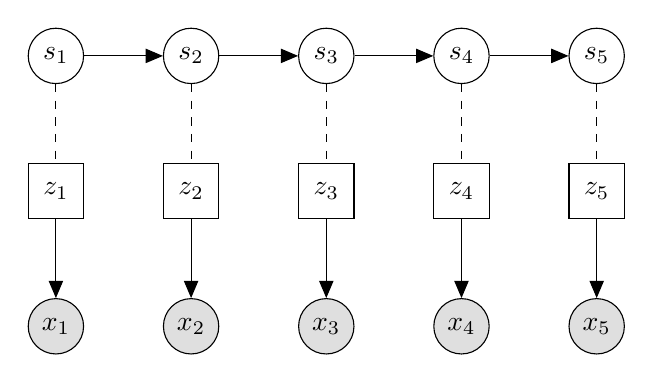
\begin{tikzpicture}

    \node[latent] (s1) {$s_1$};
    \node[latent, right=of s1] (s2) {$s_2$};
    \node[latent, right=of s2] (s3) {$s_3$};
    \node[latent, right=of s3] (s4) {$s_4$};
    \node[latent, right=of s4] (s5) {$s_5$};
    \node[latent, rectangle, below=of s1] (z1) {$z_1$};
    \node[latent, rectangle, below=of s2] (z2) {$z_2$};
    \node[latent, rectangle, below=of s3] (z3) {$z_3$};
    \node[latent, rectangle, below=of s4] (z4) {$z_4$};
    \node[latent, rectangle, below=of s5] (z5) {$z_5$};
    \node[obs, below=of z1] (x1) {$\Matrix{x}_1$};
    \node[obs, below=of z2] (x2) {$\Matrix{x}_2$};
    \node[obs, below=of z3] (x3) {$\Matrix{x}_3$};
    \node[obs, below=of z4] (x4) {$\Matrix{x}_4$};
    \node[obs, below=of z5] (x5) {$\Matrix{x}_5$};

    \edge{s1}{s2};
    \edge{s2}{s3};
    \edge{s3}{s4};
    \edge{s4}{s5};
    \edge[dashed,-]{s1}{z1};
    \edge[dashed,-]{s2}{z2};
    \edge[dashed,-]{s3}{z3};
    \edge[dashed,-]{s4}{z4};
    \edge[dashed,-]{s5}{z5};
    \edge{z1}{x1};
    \edge{z2}{x2};
    \edge{z3}{x3};
    \edge{z4}{x4};
    \edge{z5}{x5};

\end{tikzpicture}

\end{document}
